%
% The Current Maintainer of this work is Paul Vojta.

\documentclass[masters]{ucbthesis}
\usepackage{biblatex}
\usepackage{color}
\usepackage{graphicx}
\usepackage{subcaption}
\usepackage{siunitx}
\usepackage{listings}
\usepackage{rotating}
\usepackage{multirow}
\usepackage{xspace}

% To compile this file, run "latex thesis", then "biber thesis"
% (or "bibtex thesis", if the output from latex asks for that instead),
% and then "latex thesis" (without the quotes in each case).

% Double spacing, if you want it.  Do not use for the final copy.
\def\dsp{\def\baselinestretch{1.5}\large\normalsize}
\dsp

% If the Grad. Division insists that the first paragraph of a section
% be indented (like the others), then include this line:
% \usepackage{indentfirst}

% commands
\newcommand{\ignore}[1]{}
\newcommand{\TODO}[1]{{\color{red}\textbf{TODO: #1}}}
\newcommand{\RISCV}{\mbox{RISC-V}}
\newcommand{\wunits}[2]{\mbox{#1\,#2}}

% commands use to alias tbd names
% Paper name
\newcommand{\PNAME}{\mbox{\textsc{fased}}\xspace}
% Simulation framework name
\newcommand{\SIMNAME}{MIDAS\xspace}

\bibliography{refs}

% Increase the depth of numbering sections

\hyphenation{Rocket-Chip MIDAS}
\begin{document}

% Declarations for Front Matter

\title{An FPGA-Hosted Reconfigurable Timing-Model For Joint Last-Level-Cache And DDR-SDRAM Memory Systems}
\author{David Thomas Biancolin}
\degreesemester{Spring}
\degreeyear{2018}
\degree{Master of Science}
\chair{Professor Krste Asanovi\'c}
\othermembers{Professor Jonathan Bachrach}
\numberofmembers{2}
% Previous degrees are no longer to be listed on the title page.
% \prevdegrees{B.A. (University of Northern South Dakota at Hoople) 1978 \\
%   M.S. (Ed's School of Quantum Mechanics and Muffler Repair) 1989}
\field{Electrical Engineering and Computer Science}
% Designated Emphasis -- this is optional, and rare
% \emphasis{Colloidal Telemetry}
% This is optional, and rare
% \jointinstitution{University of Western Maryland}
% This is optional
\campus{Berkeley}

% For a masters thesis, replace the above \documentclass line with
% \documentclass[masters]{ucbthesis}
% This affects the title and approval pages, which by default calls this
% document a "dissertation", not a "thesis".

% A slightly modified template of the ms thesis to reuse the title variables
\clearpage
\makeatletter
\thispagestyle{empty}

\begin{center}
\rule{6.5in}{0.40mm}

\vspace{0.35in}
    {\large \textbf{\@title} }

\vspace{0.25in}
    {\large by \@author }

\vspace{0.35in}
\rule{6.5in}{0.40mm}

\vspace{0.5in}
    {\large {\textbf{Research Project}}}
\end{center}

\noindent Submitted to the Department of Electrical Engineering and
Computer Sciences, University of California at Berkeley,
in partial satisfaction of the requirements for the degree
of \textbf{Master of Science, Plan II}.

\vspace{0.25in}
\noindent Approval for the Report and Comprehensive Examination:

\begin{center}
    \textbf{ Committee:}

\vspace{0.25in}
\rule{3.5in}{0.25mm}

\@chair

Research Advisor

\vspace{0.25in}
\rule{3.5in}{0.25mm}

(Date)

\vspace{0.25in}
* * * * * * *

\vspace{0.25in}
\rule{3.5in}{0.25mm}

\@othermembers

Second Reader

\vspace{0.25in}
\rule{3.5in}{0.25mm}

(Date)
\end{center}
\makeatother

\maketitle
% Delete (or comment out) the \approvalpage line for the final version.
%\approvalpage
%\copyrightpage

%Recent work in FPGA-accelerated simulation of ASICs has shown that much
of a simulator can be automatically generated from ASIC RTL.  Alas, these works rely on simple models of
the outer cache hierarchy and DRAM, as
mapping ASIC RTL for these components into an FPGA fabric is too
complex and resource intensive.  To improve FPGA simulation model
accuracy, we present \PNAME~(FPGA-Accelerated Simulation and Evaluation of DRAM), a
parameterized generator of composable, high-fidelity, FPGA-hosted
last-level-cache and DRAM models. \PNAME instances are highly
performant, yet they maintain timing faithfulness independently of the
behavior of the host-FPGA memory system.
For a given scheduling policy, a single \PNAME instance can model
nearly the entire space of realizable single-channel DDR3 memory
organizations, without resynthesizing the simulator RTL.
We demonstrate \PNAME by integrating it into a flow that automatically
transforms RTL for multicore RISC-V processors into full-system
simulators that execute at up to 150 target MHz on cloud-hosted FPGAs.


\begin{frontmatter}

% You can delete the \clearpage lines if you don't want these to start on
% separate pages.

\setcounter{tocdepth}{2}
\setcounter{secnumdepth}{2}
\tableofcontents
\clearpage
\listoffigures
\clearpage
\listoftables

    \begin{acknowledgements}

I'd like to thank my advisors, Jonathan Bachrach and Krste Asanovi\'c, for
their guidance and immesurable patience; my collaborators for their assistance in
bringing this paper --- my first, first-author publication --- to
fruition; and my girlfriend and family for their steadfast belief in me.

    \end{acknowledgements}
\end{frontmatter}

\pagestyle{headings}

% (Optional) \part{First Part}
\begin{abstract}
Recent work in FPGA-accelerated simulation of ASICs has shown that much
of a simulator can be automatically generated from ASIC RTL.  Alas, these works rely on simple models of
the outer cache hierarchy and DRAM, as
mapping ASIC RTL for these components into an FPGA fabric is too
complex and resource intensive.  To improve FPGA simulation model
accuracy, we present \PNAME~(FPGA-Accelerated Simulation and Evaluation of DRAM), a
parameterized generator of composable, high-fidelity, FPGA-hosted
last-level-cache and DRAM models. \PNAME instances are highly
performant, yet they maintain timing faithfulness independently of the
behavior of the host-FPGA memory system.
For a given scheduling policy, a single \PNAME instance can model
nearly the entire space of realizable single-channel DDR3 memory
organizations, without resynthesizing the simulator RTL.
We demonstrate \PNAME by integrating it into a flow that automatically
transforms RTL for multicore RISC-V processors into full-system
simulators that execute at up to 150 target MHz on cloud-hosted FPGAs.

\end{abstract}

\chapter{Introduction}

\chapter{Introduction}



% Sagar: stylistic, but I don't like this section title vs just "Background" or something
\chapter{On FPGA-based Simulation}

% This section describes historical and related FPGA simulation work, and aims
% to call out techniques employed by this paper, in addition to describing
% problems with those works

We first review the use of FPGAs for architecture studies.  Throughout
this paper, we make a distinction between the \emph{target} and
the \emph{host}.  The target is the design under study.  Combining the
target with a model of the environment in which it executes forms a
determinate closed system whose behavior is defined independently of
the simulation host.  The host is the hardware that
executes~(\emph{hosts}) the simulation.  In this paper, a host
consists of one or more CPUs connected to one or more FPGAs.

\section{FPGA Prototyping}
FPGAs have long been used to \emph{prototype} ASICs by implementing
the ASIC RTL directly in FPGA logic.  While FPGA prototypes are both
fast~(10s to 100s of MHz) and detailed, they require a complete RTL
description of the target design. Furthermore, larger designs must be
painstakingly partitioned across multiple FPGAs. Since these
multi-FPGA prototypes advance in lockstep, cycle by cycle, they are
considerably slower~(100s of KHz to 1s of MHz). Nonetheless, FPGAs are used widely
in industry, as they allow software development and hardware
validation to proceed months before silicon is available.

\section{FPGA-Accelerated Simulation}

Prior work has explored techniques to make FPGAs more usable and
powerful simulation hosts.  Motivated by the dawn of the multicore
era, the multi-university RAMP project~\cite{RAMP} made large strides
in improving FPGA-accelerated simulators by improving resource
efficiency, developing FPGA partitioning techniques, and avoiding FPGA
recompilation by using reconfigurable models.

ProtoFlex~\cite{protoflex} was an architecture-level simulator that
demonstrated 16-way host-multithreading of a single FPGA-hosted functional model.
ProtoFlex could switch between FPGA-hosted and CPU-hosted modes via
\emph{transplantation}. FAST~\cite{FAST}, a cycle-accurate simulator, was
split into CPU-hosted functional and FPGA-hosted timing models.  RAMP
Gold~\cite{RAMPGold} used FPGA-hosted timing and functional models
with 64-way host-multithreading to model a larger target on a single
FPGA.  HAsim~\cite{HASIM} also used FPGA-hosted timing and functional
models, but provided more detailed pipeline and memory hierarchy
models.

Other work studied partitioning targets over multiple FPGAs.
\cite{LIFPGADesign} showed that by partitioning HAsim over two FPGAs, they
could model eight times as many cores, due to improved resource sharing between
virtual instances. To model a datacenter-scale target, DIABLO~\cite{Diablo}
leveraged RAMP Gold's multithreading to simulate 3072 servers on 24 FPGAs.

A unifying theme of FPGA-accelerated simulators is that one clock-cycle of
target time is executed over a variable number of FPGA-host
cycles.  This lets an FPGA-hosted simulator hide
variable host latencies to DRAM and CPU-hosted components, enables
optimizations that trade host time for host resources, and, crucially,
facilitates deterministic simulation.  This \emph{host-target
decoupling} is what differentiates an FPGA-accelerated simulator from
an FPGA prototype. We expand on this property in
Section~\ref{sec:fame1}.

\section{Adoption Challenges}

Despite their promise, FPGA-accelerated simulators have only been
successfully employed by those who designed them. We attribute their
limited appeal to several factors:

\begin{enumerate}

    \item \textbf{Availability.} Much of the early FPGA-accelerated
    simulator research relied on boutique FPGA-emulation
    platforms or custom board designs, whose high cost and
    limited availability prevented adoption.

    \item \textbf{FPGA Capacity.} Common ASIC structures, such as CAMs and
        multi-ported RAMs, map poorly to FPGA
        fabrics~\cite{FPGAGap2}, making it difficult to host large
        ASIC designs on FPGAs.

    \item \textbf{Ease of Use.} To avoid partitioning across multiple
     FPGAs, previous work focused on efficiently mapping more of the
     target to a single FPGA. The abstract, multithreaded models these
     simulators typically employ can be more difficult to implement
     than the machines they model, greatly undermining their
     usability. This complexity limits configurability, forcing users
     to modify a sophisticated piece of RTL to make larger
     changes. Furthermore, these abstract models must, like their
     software counterparts, be validated and calibrated, making them
     even more laborious to use.
\end{enumerate}

\section{Recent Technological Advances}

Even as Moore's law wanes, FPGA capacity continues to scale. The largest FPGAs
have over \wunits{50}{MiB} of BRAM and millions of logic cells.
%\footnote{Scaling RAMP
%Gold~\cite{RAMPGold} to use the largest Xilinx UltraScale+
%FPGA~\cite{Ultrascale} would permit modeling more than 5000 cores!}
As they
have scaled, FPGAs have become more heterogeneous, adding features that make
them better hosts for full-system simulators.  Both Intel and Xilinx sell FPGAs
with embedded microprocessors, making it easier to co-simulate tightly coupled
hardware and software models. Modern FPGAs include dedicated DRAM
controllers that support memory bandwidths rivaling those of ASICs.

Lower cost and increased on-chip integration have also made FPGAs more
accessible to researchers.  Not only are commercial off-the-shelf development
boards cheaper and more full-featured, FPGAs are now available as a cloud service~\cite{amazonf1}.
Where in the past academics would have to purchase their own FPGAs to reproduce
published experiments, instead, it is now possible to spin up identical
simulations on FPGAs in the cloud.  This development promises to foster more
collaboration around FPGA-accelerated simulation.

\section{Usability Through Automation}

While the trends described in the previous section solve the
\emph{availability} and \emph{FPGA capacity} challenges, usability remains a
problem. Previous work~\cite{fabscalarfpga, strober} has shown that much of an
FPGA-accelerated simulator can be automatically generated from source RTL. This RTL
can be written in an HDL like Verilog, generated by a high-level synthesis
tool, or emitted by languages like Chisel~\cite{Chisel} or Bluespec.

Alas, it is not always practical to generate models from source
RTL. Consider off-chip memory systems: they are too resource-intensive to host
in the FPGA fabric, yet for reasonable simulation performance, they must be
tightly coupled with the processor model.  Components like these require
an abstract model to virtualize the target memory system over DRAM attached
to the FPGA---reintroducing the problem that anything
but a simplistic model is difficult to design, validate, modify, and reuse.

To avoid these pitfalls, we propose writing detailed memory-system
timing models as decoupled, split-timing-and-functional models with
the timing models written as \emph{target-time} RTL. Using this
approach, the same RTL transformations applied automatically to the
processor RTL are applied to the timing-model RTL before binding it to
the functional model.  Model designers can focus on modeling detailed
target behavior and not worry about the mapping to the host.  With our
approach, since timing models are transformed from target-time RTL, it
is possible to use HLS-generated RTL or even existing
memory-controller RTL as a timing model.

To improve reusability, we propose writing timing models
as \emph{generators}.  This allows the model designer to describe a
space of \emph{instances} with less development effort.  To
support reconfiguring timing models without FPGA recompilation, timing
models expose timing parameters as I/Os that are bound automatically
to memory-mapped registers during timing-model generation.  Taken
together, these techniques make it possible to describe
detailed, reusable memory-system models.  We demonstrate this claim with \PNAME.


\chapter{The Simulation Framework}\label{sec:framework}

We prototype our models in an FPGA-Accelerated simulation framework that builds on
the Rocket-Chip \cite{rocketchip} infrastructure (similar to
\cite{strober}). Our designs are developed in Chisel, a high-level
hardware-description language written in Scala. Building on this infrastructure
allows us to leverage a large amount of available open-source IP and a growing
software ecosystem that includes GCC, Linux and LLVM.

Our framework makes use of FIRRTL~\cite{firrtl}, an intermediate representation
(IR) for RTL that has frontends for both Chisel and Verilog, and can target
both FPGA and ASIC flows by emitting optimized Verilog output. FIRRTL enables
the implementation of compiler passes on top its IR framework. These passes
can, for example, apply FPGA-optimizations, add instrumentation, and
automatically produce scan chains for debugging and power
estimation\cite{strober} -- all without requiring modifications to the source
RTL.

\begin{figure}
	\centering
	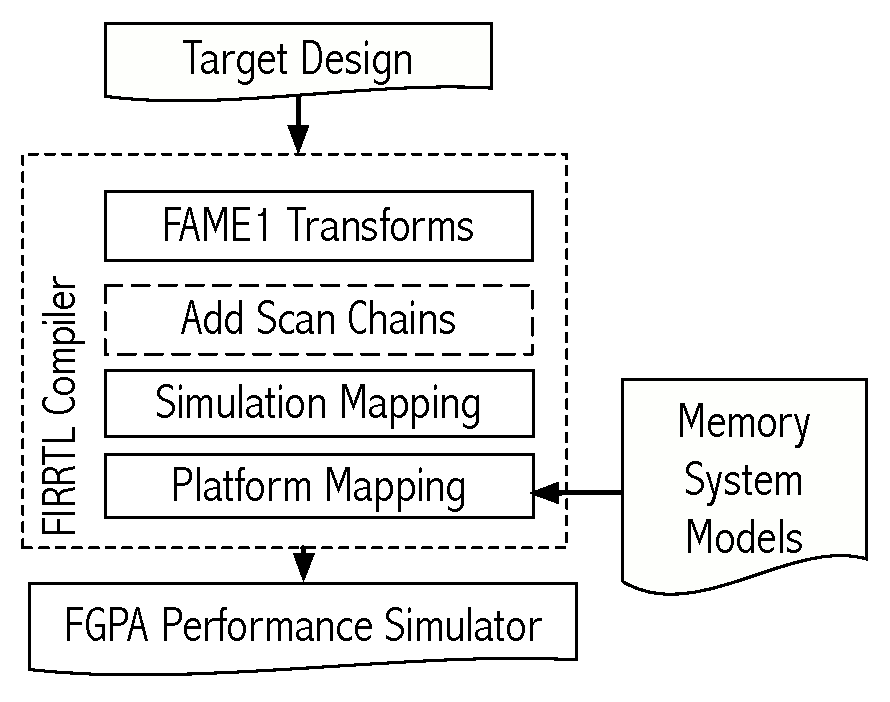
\includegraphics[width=7cm]{figures/firrtl.pdf}
	\caption{FIRRTL custom transforms for the FPGA simulator}
	\label{fig:firrtl}
\end{figure}


\section{Host-Target Decoupling in MIDAS}

\section{Transformations of Source RTL}

MIDAS uses FIRRTL compiler passes to preform transformation source RTL into
host-decoupled models. The most important of these is the FAME-1
transformation, which adds to requsite logic to host-decouple target RTL, so
that it may conform to a RAMP model of execution. \TODO{See Section}. In figure
\TODO{Auto-transformation} below, the procedure through which source RTL is
host decoupled is illustated.


Additional transformations may be invoked to add scan
chains and I/O trace buffers for debugging, and for state snapshotting for use
with Strober\cite{strober}.

\section{Platform Mapping}

\section{Target Machines}

While this approach is applicable to arbitrary RTL, one challenge lies in
sourcing the RTL to build a realistic target. While we build on RocketChip and
\RISCV, our approach could in principle be used with other open-source designs
such as OpenPiton\cite{openpiton} and FabScalar\cite{fabscalar}.


\chapter{Memory Model Architecture}

% This section describes the design of the memory system model. How host target
% decoupling is achieved. What configurations are available.

Our memory system model \textit{generator} describes a space of individual
\textit{instances} that model different memory systems. Implemented in
Chisel\cite{Chisel}, the generator emits a host-decoupled module that is
attached to other simulation models during simulation mapping. All instances
are runtime-configurable via memory-mapped registers that presented on the
MIDAS simulation interconnect.

Instances operate by using the FPGA host's off-chip memory system as a backing
store: target requests carried through simulation tokens are snooped by the
\emph{ingress unit} and re-issued to the host memory system. Reponses from the
host memory system are subsequently saved by the \emph{egress unit}.  In
parallel, a host-decoupled \emph{timing model} explicitly consumes input tokens
and generates output tokens. When the timing model wishes to release a token
with a valid target response, it fetches the matching host response from the
egress unit. If no host response is present, the timing model does not produce
a token, thus, simulation timing is maintained regardless of host-memory system
timing.

\begin{figure}
	\centering
	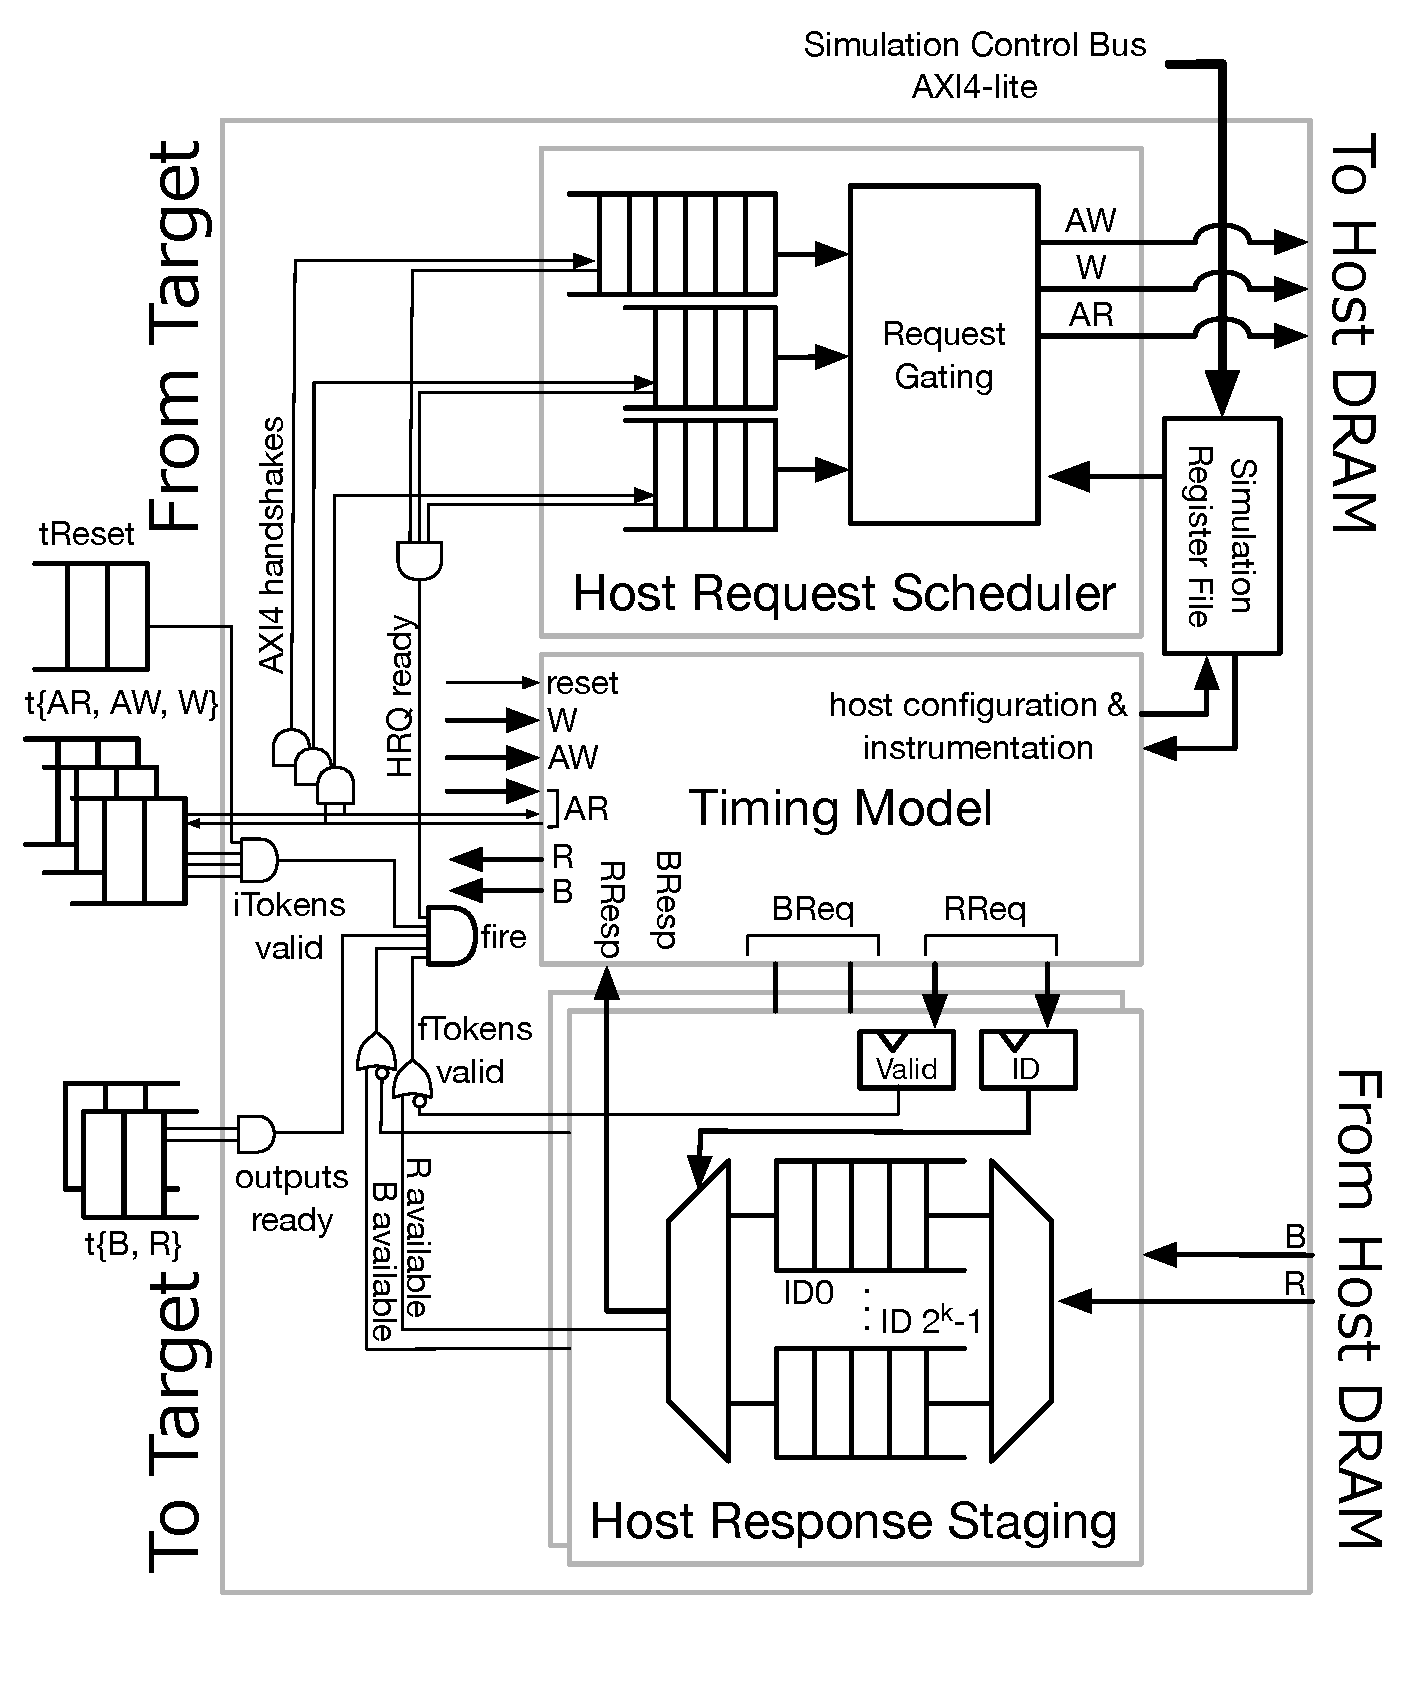
\includegraphics[width=\columnwidth]{figures/memory-model-block-diagram.pdf}
	\caption{Top-level diagram of memory system model with latency-bandwidth pipe timing model}
	\label{fig:timing_model}
\end{figure}

\section{Interfaces}

All instances of the model have three interfaces.

\begin{enumerate}
    \item \textbf{Target-Side} Host-decoupled AXI4 slave
        interface and synchronous reset. AXI4 consists of five ready-valid
        channels; three request channels driven by the master, and two
        reponse channels driven by the slave.  An input token consists of
        the valids and payloads for each request channel, the readies for
        each reponse channel, and the synchronous reset.  An output token
        is the complement; the valids and payloads for each response
        channel, and the readies for each request channel.  While tokens
        may be carried to and from the instance on seperate timing channels
        (for each AXI-4 channel and reset), simulation mapping ensures
        these are fused into a single input token, and fractured into
        multiple output tokens accordinly.

    \item \textbf{Host-Side} AXI4 master. This interface is used by the instance
        to make requests of the host memory system. It has no notion of target time.

    \item \textbf{Configuration-Side} AXI4-lite slave. This interface exposes both
        memory-mapped configuration registers and instrumentation to the
        simulation interconnect. During generation, the local memory map of the
        instance is produced and is included in the global simulation memory map
        in const.h.

\end{enumerate}

We selected AXI4 as it is the most common memory interface presented by FPGA IP
and widely implemented in ASICs. On the host-side, both major FPGA vendors
provide IP to bridge AXI4 to other standards, as well as adapters, to connect
master and slave devices that may have different interface widths. On the
target-side, the user will need to generate a bridge in their source RTL if
their design does not present and AXI4 master. In the future, we expect to
include target side interfaces for other interface specifications, like
TileLink.

The widths of all fields in target-side and host-side interfaces match, with
the exception of ARID and AWID. Here, the model can optionally reduce the
host-side ID width to the AXI4 specification's recommended maximum (4) or tie
it off altogether to prevent host-memory system reorderings. The model punts on
all other conversions, like target-to-host address translation, which will be
handled by the MIDAS compiler.

\section{Functional-Timing Split}

Like most previous FPGA-simulation work using custom RTL models, the generator
employs a timing-functional split. The egress and ingress units are functional:
they "emulate" target-memory system requests over a region of the host-memory
system of equal size. These units operate independently of target time and are
reused across all timing model classes. As the name suggests, the timing split
is captured entirely in the timing model.

The timing model interacts with the functional units in two places. Firsly,
through the simulation-side interface. Secondly, through the egress
request/response interface. Here, the timing model presents an AXI4 ID for the
host reponse it wishes to release to the target. The egress unit will reply
with the reponse if it is available, the timing model must fully dequeue the
reponse before requesting another\footnote{The AXI4 specification does not
permit interleaving of multiple read responses.}.

\begin{figure*}
	\centering
	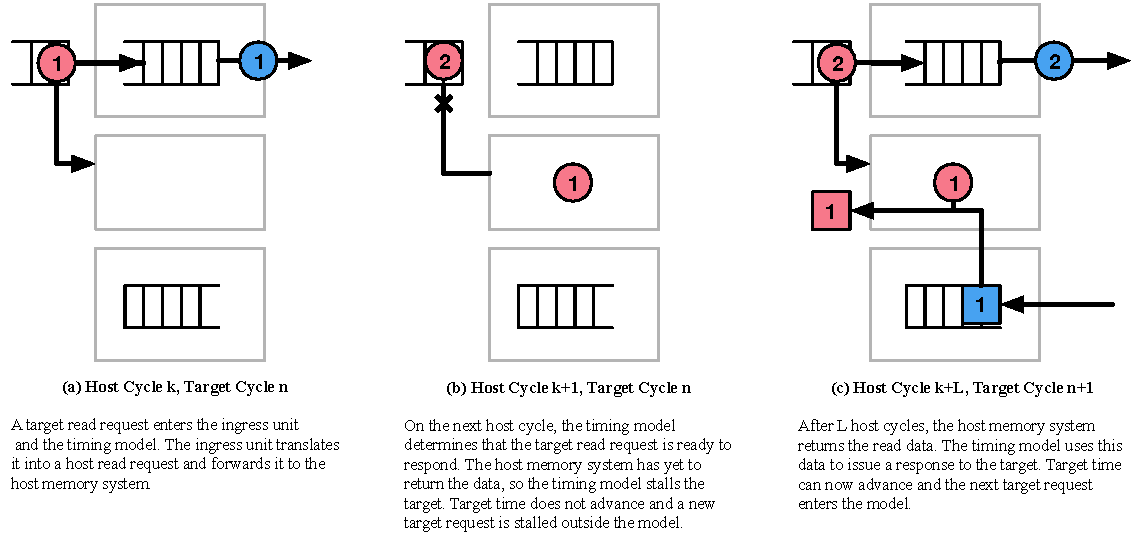
\includegraphics[width=0.8\textwidth]{figures/memory-model-operation.pdf}
	\caption{Operation of a single-cycle "magic" memory}
	\label{fig:model_operation}
\end{figure*}

\subsection{Egress Unit Design}\label{egress} Since both the host memory
system and the timing model may reorder responses\footnote{The AXI4
specification permits reordering of read and write responses across different
channels(different AXI4 IDs). Reponses within a particular channel must be
returned in the order they were requested. AXI4 imposes no ordering timing
constraints between read and write requests.} the egress unit implements a set
of virtual queues for each AXI4 channel. Each queue represents the FIFO
ordering within a single channel ID. The implementation of the virtual queues
differs based on:

\begin{itemize}
    \item Maximum number of outstanding requests
    \item Maximum number of AXI4 channels used by outstanding requests
    \item Minimum and maximum read request length
\end{itemize}

For a small number of IDs or a small number of outstanding requests, the
memory system model implements each virtual queue as a physical queue co-located in
the same BRAM. For greater numbers of AXI IDs, it dynamically assigns entries
within the BRAM to each response and maintains a list of pointers to those
entries for each channel ID.

\section{Configurability}

There are two points at which the model can be configured.  At
\textit{generation time}, the designer selects an instance. At
\textit{simulation time}, the instance is programmed through its
configuration-side interface to further set its behavior. Simulation time
configurability permits the designer to perform parameter sweeps without
needing to recompile the simulator bitstream -- at the expense of FPGA
resources. Since both timing and functional components of an instance are
provisioned pessimistically, giving hints to generator can greatly reduce FPGA
resource utilization. We outline some programmability-area tradeoffs here.

\begin{itemize}
    \item \textbf{Reducing functional component size.} The simulation designer
        can call out constraints on the behavior of the AXI masters to reduce
        the size of the ingress and egress units.  This achieved by putting
        bounds on the parameters defined in \ref{egress}.

    \item \textbf{Selecting the timing model class.} Simpler timing models
        consume fewer resources.

    \item \textbf{Reducing model programmability.} By default, each timing
        model class exposes all of its parameters as programmable registers on
        the simulation memory map. The generator permits tying particular knobs
        to static values, saving FPGA resources.

    \item \textbf{Reducing model instrumentation.} Model instances can be
        generated with instrumentation to track specific events and capture
        activity traces. This instrumentation is exposed on the simulation
        memory map. Generating the model with less instrumentation uses fewer
        resources.
\end{itemize}

\section{Timing Model Classes}\label{sec:timing_model}

The generator provides four base timing model classes:

\begin{itemize}
    \item \textbf{Latency-Bandwidth Pipe} Applies independently programmable
        latencies to read and write requests. The pipe does not accept any new
        requests beyond a programmable limit. This serves as a coarse-grain
        bandwidth bound via Little's law.

    \item \textbf{Bank Conflict} Adds a penalty of $max(0, t_{CP} -
        t_{\Delta})$ to a base latency if a read or write request used the bank
        $t_{\Delta}$ cycles prior, where $t_{CP}$ is the maximum conflict
        penalty.

    \item \textbf{FCFS DRAM MAS} Implements \ref{fcfs} with configurable open
        and closed page policy.

    \item \textbf{FR-FCFS DRAM MAS} Implements \ref{frfcfs} with an open page
        policy.
\end{itemize}

\TODO{Programmability charts}

Note that while the latter two models do have programmable $t_{RP}$, $t_{CS}$,
$t_{RCD}$, they are incomplete models of a generic DDR DRAM. For example, they
do not check against all DRAM timing constraints, nor do they model refresh.
They do, however, significantly improve modeling fidelity of DRAM memory
systems (with their respective MASs). We expect that the latency-bandwidth pipe
and bank conflict model will also suffice for modeling a slew of other memory
technologies to a first-order approximation.



\chapter{On DRAM Memory Systems}

\section{DRAM Device Architecture}\label{sec:dram-arch} In a DRAM IC, arrays of
bit cells are hierarchically arranged into multiple parallel \emph{banks}.
Banks provide the primitive level of concurrency in a DRAM memory system. They
can service independent requests, assuming they do not simultaneously require
shared resources like the data, address and command buses.  Multiple DRAM ICs
can be arranged in parallel to widen the data bus; address and command buses
fan out to each IC. For more concurrency, and to support larger memory
capacities, multiple \emph{ranks} of DRAM devices may be used. Here, generally,
the command and data buses are shared between all ranks, with a one-hot
chip-select indicating which rank a command is addressed to.

A basic DRAM operation requires a series of three commands: \emph{activate
(ACT)}, \emph{column access~(CAS)}, and \emph{precharge~(PRE)}. The ACT command
enables the word-lines of the array corresponding to a single \emph{row} of the
bank. The cells of the row are sensed and saved in a \emph{row
buffer}(typically 1-2 kB). A CAS command then selects a subset of the row
buffer to read or write~(CASR and CASW commands respectively). In double-data
rate~(DDR) DRAM, data is bursted over successive rising and falling clock
edges.  While the row buffer remains \emph{open}, the row can be accessed by
issuing new CAS commands. To access a row not stored in the buffer, a PRE
command must be issued to \emph{close} the row and charge the bit lines for a
new access.

DRAM is named dynamic-RAM because it gradually loses its stored state over time
as bit-cell capacitors leak. DRAM-cell retention rates vary on a single die and
between dies and are highly sensitive to temperature~(warmer cells leak
faster). To maintain their state, DRAM cells must be periodically ``refreshed".
Activating a row of cells is sufficient to refresh them: the stored state is
read by the sense amplifiers and fed back into the bitlines at the supply
voltage, recharging the still-open capacitors.  As part of the DRAM standards,
JEDEC mandates cells must be refreshed on-average once every 8ms; an interval
they have maintained from DDR through DDR4. Since activations to every row
cannot generally be guaranteed, DRAM devices are refreshed explicitly with
a refresh command~(REF). To reduce complexity, this command refreshes a constant
number of contiguous rows beginning at a base row address in all banks
concurrently. The base address is incremented which each REF command. DRAM manufacturers generally
have kept the number of refresh commands required to iterate through the entire
array constant: 8192 commands per 8ms interval, or one on average every 64 $\mu s$.
Hence, refresh commands take longer to execute on denser devices with more rows
per bank.

A complete list of timings required to model a generic DDR protocol is give in
table \ref{tbl:dram-timings}. These have been taken, with some modification,
from \textit{Memory Systems: Cache, DRAM, Disk}\cite{drambook}.

\begin{table}[htb]
\begin{center}
\resizebox{\textwidth}{!}{%
    \begin{tabular}{|p{0.20\textwidth}|p{0.8\textwidth}|}
    \hline
    \textbf{Name} & \textbf{Description} \\
    \hline
    \hline
    \textbf{$t_{AL}$} & Additive Latency. Additional latency added to column access commands. \\
    \textbf{$t_{CAS}$~($t_{CL}$)} & Column Access Strobe latency. Delay between
    when a CASR command is received and when the first beat of read data is
    returned. \\ \textbf{$t_{CCD}$} & Column-to-Column Delay. Minimum duration
    between two consecutive column commands. \\ \textbf{$t_{CMD}$} & Command
    transport duration. The duration a command occupies the command bus. \\
    \textbf{$t_{CWD}$~($t_{WL}$)} & Column Write Delay. The delay between a
    CASW command and the when the controller must present the first beat of
    write data. \\
    \textbf{$t_{FAW}$} & Four row Activation Delay. A rolling time window
    during which only four row activations may be made to all banks of a DRAM
    device. \\
    \textbf{$t_{RAS}$} & Row Access Strobe. The minimum duration after an ACT
    command that the row must be kept open before issuing a precharge command
    to close it. \\
    \textbf{$t_{RC}$} & Row Cycle time. The minimum duration required
    to open, and close a row. $t_{RC} = t_{RAS} + t_{RP}$ \\
    \textbf{$t_{REFI}$} & Refresh Interval. The average period of time between refresh commands. \\
    \textbf{$t_{RCD}$} & Row-to-Column Delay. The minimum duration after
    activation column commands may be issued to the newly-opened row.  \\
    \textbf{$t_{RFC}$} & ReFresh Cycle time. The minimum duration after a refresh
    command that activation commands may be issued. \\
    \textbf{$t_{RP}$} & Row Precharge delay. The minimum duration after a
    precharge command that an ACT to the same bank may be issued. \\
    \textbf{$t_{RRD}$} & Row-to-Row Delay. The minimum duration between ACT commands to the same bank. \\
    \textbf{$t_{RTP}$} & Read-To-Precharge delay. The mimimum duration after a CASR command that a precharge may be issued to the same row. \\
    \textbf{$t_{RTRS}$} & Rank-To-Rank Switching delay. Accounts for time to change termination schemes on DQ and DQS buses when switching between ranks. \\
    \textbf{$t_{WR}$} & Write Recovery time. The minimum duration after a CASW command that a precharge command may be issued to the same row. \\
    \textbf{$t_{WTR}$} & Write TurnaRound Time. The minimum duration after a CASW command that a CASR may be issued to the same row. \\
    \hline
\end{tabular}}
\end{center}
\caption{A list of key timings for a conventional DDRx SDRAM}
\label{tbl:dram-timings}
\end{table}%

\clearpage
\section{DRAM Controller Architecture}

A DRAM controller is responsible for responding to memory
requests from one or more requestors by scheduling those requests over its
attached memories as a judicious stream of DRAM commands.

Memory access scheduling~(MAS) is the process by which, for a given cycle, a
controller selects a single DRAM command to be issued from a legal set. Legal
commands are constrained by the current state of each bank, the availability
of shared resources like the command and data buses, and timing constraints
imposed by the DRAM standard. Good MAS policies strike a delicate balance
between minimizing latency, maintaining quality-of-service guarantees across
multiple threads of execution, maximizing bandwidth, and minimizing power.
There are plethora of academic papers on MAS policies, and still more
industrial patents on the subject. In this work we consider two popular MAS policies. 

\subsection{First-Come First-Serve~(FCFS) Policy}\label{sec:fcfs} Commands for the
oldest pending memory reference are issued first. This is the simplest MAS
policy, but tends to under-utilize available DRAM bandwidth as younger requests
that may hit in the row-buffer are not issued before older commands that miss.
FCFS schedulers are common in older machines, and those that present few
concurrent memory requests.

\subsection{First-Ready FCFS~(FR-FCFS)~\cite{frfcfs} Policy}\label{sec:frfcfs}
First, ready~(legally issuable) column commands are prioritized over ready row
commands. Second, commands for older references are prioritized over younger
ones. This permits younger but ready column commands to be issued before older
row commands. FR-FCFS is a relatively simple scheme that improves bandwidth
utilization considerably. It is the de facto standard against which new MAS
policies for machines with a single stream of memory references~(like
single-core out-of-order machines), are compared.

\section{DRAM Software Simulation}

The current state of the art in DRAM simulation in academia are cycle-accurate
software simulators like DRAMSim2~\cite{dramsim}, Ramulator~\cite{ramulator} and
USIMM~\cite{usimm}. These models generate DRAM command streams that have been
validated against industrial models~(for some standards). Both Ramulator and
DRAMSim2 can be easily integrated into Gem5~\cite{gem5}, though gem5 includes a
detailed event-based model of its own~\cite{gem5event}. In trace-driven mode,
operating at full throughput and only as a timing-model, these cycle-accurate
models simulate at frequencies ranging from hundreds of KHz to ones of
MHz~\cite{ramulator}.

\section{DRAM Power Modeling}

In order to model power, Ramulator relies on DRAMPower~\cite{drampower}, to
which it passes its command trace. DRAMSim2 directly implements strategies
Micron has described in their technical notes~\cite{micronpower}. Micron has
also provided spreadsheets implementing these strategies, that take
microarchitectural event frequencies as input. These approaches can also be
used in an FPGA simulation, as sufficiently detailed FPGA models can add
instrumentation for specific events, while simpler models could save or sample
the memory access trace and compute power out-of-band.


\chapter{DRAM Timing Models}\label{sec:dram-timing-model}

We provide two DDR3 timing-model classes based around FCFS and FR-FCFS MAS.
DDR3 timing models have a runtime-configurable address assignment, speed grade,
page policy, and rank, bank, and row count. The timing models generate legal
DDR3 command traces that have been validated against Verilog golden models.

\section{Timing Model Design}
Both timing-model classes consist of four components: transaction
scheduler, DRAM state trackers, MAS, and backend.

\subsection{Transaction Scheduler}
The transaction scheduler consists of a single, unified, configurable-depth
queue that can accept an AXI4 read and write transaction simultaneously. Reads
are given priority when only one slot is available.  Transactions are passed to
the MAS as they can be accepted at a rate of one transaction per cycle.

\subsection{DRAM State Trackers}
We decoupled the MAS model design from structures that track the state
of DRAM devices. The DRAM state tracker is arranged hierarchically into rank and
bank state trackers. State trackers present to the MAS a bit vector indicating
which commands they may legally accept. Trackers have a counter for each command
type, which indicate the next earliest cycle that the tracker can legally accept a command of
that type. When the MAS issues a command, it informs the associated state tracker,
which updates its counters accordingly.

\subsection{Memory Access Scheduler}
Each MAS maintains a data structure of memory references it is scheduling across.
When a new transaction is received, a record in this structure is populated with the decoded rank, bank, and row addresses, along with
MAS-specific metadata to ease scheduling decisions.
On every target cycle, the MAS
selects a legal command based on the available references and the bit vectors
presented by the state trackers. The MAS releases reads to the backend on the
cycle the first beat would return from DRAM. Writes are released the cycle after a
CASW command is issued.  Both MAS models have a simple, runtime-configurable
page policy. The open-page policy keeps pages open until the next refresh or another row
is to be opened. The closed-page policy always issues auto-precharged CAS
commands. To maintain a global age-order of memory references, the FR-FCFS MAS
uses a single collapsing buffer with a runtime-programmable depth.

\subsection{Refresh Policy}
Both MAS use an interrupting, all-ranks refresh scheme that makes no attempt to
pull-in or delay refresh commands.  When a refresh is requested, the MAS
precharges all banks in all ranks, and issues REF commands as soon as possible.

\subsection{Backend}
The backend receives read and write references from the MAS and drives the AXI4
response channels back to the target. If no LLC is being used, read response data is fetched from the host-response staging unit.
The backend can apply an additional runtime-configurable latency to simulate
additional latency on read responses and write acknowledgments.

We give the FPGA resource utilization for a handful of representative DDR3
instances in Table~\ref{tbl:dram-model-resources}.

\begin{table}[htb]
\centering
    \begin{tabular}{c c c c c}
	\hline
        \textbf{Example Instance} & LUTs & FFs & BRAM & $f_{MAX}$ \\
	\hline
        FCFS Single Rank~(SR)    & 2272 & 1647 & 1 & 272 \\
        FCFS Quad Rank~(QR)    & 4433 & 3263 & 1 & 219 \\
        FR-FCFS, SR, 8 Deep & 3172 & 2188 & 5 & 239 \\
        FR-FCFS, QR, 16 Deep & 8206 & 4805 & 1 & 158 \\
	\hline
	\end{tabular}
    \caption{Resource counts and best-case $f_{MAX}$ for four different DDR3
    models. The last instance can schedule over 16 references and thus has a larger functional model.}
\label{tbl:dram-model-resources}
\vspace{-0.35in}
\end{table}

\section{Validation}
Since our DRAM-timing models generate DRAM-command traces, we validated
traces collected in RTL simulation against a Micron DDR3 golden model. The golden
model simulates a single-device slice of the memory organization and detects
DRAM timing violations in the command trace.  We made small modifications to
the provided test bench to support validation of multi-rank organizations and
to accept our trace format. This is the same validation approach used by all
popular software cycle-accurate simulators.
To perform performance validation, we generated memory-reference traces for
which we could estimate bandwidth and row buffer hit rates a priori. The traces
were tailored to expose different memory-access scheduling behavior in the MAS
models.

\section{Selecting Legal Runtime Configurations}
Our most sophisticated DDR3 timing-model instances expose over thirty
runtime-programmable settings that specify the low-level DRAM timings,
address-assignment scheme, LLC-model configuration, and MAS-structure sizes.
Each of these settings has a legal range of values that depends on hardware in
the generated instance. To make it easier to program instances, we provide a
runtime-configuration utility that assigns these settings
from higher-level free parameters.
Users specify the DRAM data-bus width,
device DQ width, number of ranks, and total DRAM capacity. Our utility
then searches for a DDR3 device in a database and chooses one with an appropriate
density and speed grade for that memory system.

\section{Comparison to DRAMSim2} \PNAME models nearly all of the same
aspects of DRAM as DRAMSim2, but it is lacking support for burst
chopping and for power-down and self-refresh modes.
We plan to add these features in the future. \PNAME does not natively model
multi-channel memory systems, as this can be easily accomplished by using
multiple instances. Similarly, \PNAME does not natively simulate a clock-domain
crossing between the controller and the rest of the processor, instead, this is modeled in the MIDAS-generated channels.  \PNAME makes up for these
limitations with simulation speed: as part of a full-system
simulator \PNAME executes  100x - 1000x faster than popular cycle-accurate
simulators running standalone (measured in~\cite{ramulator})! We expand on
\PNAME's performance in Section~\ref{sec:evaluation}.


\chapter{Experimental Setup}

\section{Target Design Configuration}

To demonstrate of the use of our generator, we evaluated two
microarchitecturally different processors:  Rocket, a 5-stage single-issue
in-order core, and BOOM, a superscalar out-of-order core~\cite{boom}. Both
microarchitectures leverage the open-source Rocket-Chip SoC
generator~\cite{rocketchip}. As described in section~\ref{sec:targetandhostmachines}, all of the instances of RocketChip used in
this report have same top-level I/O and are modeled as part of a target with
the MIDAS SDF network shown in figure~\ref{fig:default-target}.

Both cores implement the 64-bit scalar RISC-V ISA~\cite{Waterman:EECS-2016-118,
Waterman:EECS-2016-161}\footnote{User level specification v2.1, privileged
specification v1.9} which includes support for atomics, IEEE 754-2008
floating-point, and page-based virtual memory (RV64IMAFD).
Table~\ref{tbl:target} lists the selected configurations of the target
processors.\footnote{Note that BOOM-2w roughly approximates the configuration
of the ARM Cortex-A9 processor, which coincidentally is same microarchitecture
embedded in the Zynq host.}. Unfortunately, neither configuration includes an
L2 cache as it was  temporarily removed in the version of RocketChip used to
conduct the evaluation. As a final note, the Rocket configuration we used
includes a non-blocking data cache (instead of the default blocking
implementation). Unlike a classic RISC pipeline, Rocket's backend includes a
scoreboard that allows it to make multiple memory requests when there are no
intermediate dependent instructions.

\begin{table}
\begin{center}
\resizebox{0.6\textwidth}{!}{%
\begin{tabular}{|r|c c|}
    \hline
     & \textbf{Rocket} & \textbf{BOOM-2w} \\
    \hline
    \textit{Fetch-width} & 1 & 2 \\
    \textit{Issue-width} & 1 & 3 \\
    \textit{Issue slots} & - & 16 \\
    \textit{ROB size} & - & 48 \\
    \textit{Ld/St entries} & - & 16/16 \\
    \textit{Physical registers} & 32(int)/32(fp) & 110 \\
    \textit{Branch predictor} & - & tage \\
    \textit{MSHR entries} & 2 & 6 \\
    \textit{L1 I\$ and D\$} & \multicolumn{2}{c|}{16KiB / 16KiB} \\
    \textit{ITLB and DTLB reaches} & \multicolumn{2}{c|}{128KiB / 128KiB} \\
    \hline
\end{tabular}}
\end{center}
\caption{Processor Parameters}
\label{tbl:target}
\end{table}%

%\begin{table*}
%\centering
%	\begin{tabular}{|c|S[table-format=5]|c|S[table-format=5]|c|S[table-format=5]|c|S[table-format=5]|c|}
%	\hline
%	& \multicolumn{2}{c|}{\textbf{Latency-Bandwidth Pipe}} & \multicolumn{2}{c|}{\textbf{Bank Conflict Model}} & \multicolumn{2}{c|}{\textbf{FIFO MAS}} & \multicolumn{2}{c|}{\textbf{FR-FCFS}} \\
%	\hline
%	\textbf{Resource} & \textbf{Utilization} & \textbf{\%} & \textbf{Utilization} & \textbf{\%} & \textbf{Utilization} & \textbf{\%} & \textbf{Utilization} & \textbf{\%} \\
%	\hline
%	\textit{LUT} & 3586 & 1.6 & 4170 & 1.9 & 3812 & 1.7 & 6822 & 3.1 \\
%	\textit{LUTRAM} & 651 & 0.9 & 607 & 0.8 & 655 & 0.9 & 693 & 1.0 \\
%	\textit{FF} & 3146 & 0.7 & 3929 & 0.9 & 3426 & 0.8 & 5282 & 1.2 \\
%	\textit{BRAM} & 11 & 2.0 & 11 & 2.0 & 11 & 2.0 & 11 & 2.0 \\
%	\hline
%	\end{tabular}
%
%\caption{Resource utilization of various memory system models for Xilinx zc706 FPGA}
%\label{tbl:utilization}
%\end{table*}

\section{System Software}

Unless otherwise stated, all benchmarks were run on Linux (kernel version
4.6.2). Unfortunately, at time of writing we do not have the ability to proxy a
block device requests over the tether (as is done with I/O). Thus for each
workload, we built a minimal BusyBox image and included all required files for
that workload within the image's initramfs.  Generally, workloads were compiled
statically (using \texttt{gcc -02}). When required, namely for the Java workloads, we
built library dependencies using the Yocto (\texttt{riscv-poky}) Linux
distribution generator. After packaging up the complete linux image, it is
built into an instance of the Berkeley Bootloader (BBL).

Despite our best efforts, this process produces relatively large BBL instances
($>$ 10MiB), which are slow to load directly over the tether.  We modified
\texttt{riscv-fesvr} to permit the MIDAS master to detect and accelerate program load
out-of-band (instead of fully simulating the process over the tether).

Finally, present limitations regarding how console I/O is proxied to
\texttt{riscv-fesvr} can dramatically slow down simulation depending on the
volume of target console I/O. \footnote{Changes introduced to
\texttt{riscv-fesvr} with the priviledge specification 1.10 updates remove this
bottleneck, as the host is no longer is required to acknowledge console
output.} To circumvent this, all console output is piped to a file on the
target's filesystem. At the end of the workload, the file is dumped to the
console, and \texttt{riscv-fesvr} enters a custom fast I/O mode.  Thus, low FMR
is maintained without pertubing program execution. In our evaluation flow, no
console input is ever presented to the target; the \texttt{init} script of the
linux image includes all of the commands required to run and measure the
desired workload, afterwhich it powers down the machine (See listing~\ref{lst:init} for an example).\\

\lstdefinestyle{init}{
    frame=lines,
    captionpos=b,
    %xleftmargin=\parindent,
    language=bash,
    showstringspaces=false,
    basicstyle=\footnotesize\ttfamily,
    %keywordstyle=\bfseries\color{green!40!black},
    commentstyle=\itshape\color{blue},
    identifierstyle=\color{black},
    stringstyle=\color{orange},
}

\lstset{style=init}

\begin{lstlisting}[caption={An example init script generated during the build process},label={lst:init}]
    cd /biancolin
    # Periodically polls HPM counters to measure target events
    /biancolin/rv_counters/rv_counters >> dump &
    sleep 1

    # Run the workload
    ./hello >> dump 2>&1

    # Cleanup, kill the counter program, and cat results to console
    killall rv_counters
    while pgrep rv_counters > /dev/null; do sleep 2; done
    sync
    cat dump
    poweroff -f
\end{lstlisting}

\section{Measuring the Target}

Measurements of the target design occur in two places.
Memory timing-model instances collect their own statistics, and
as described previously, are read with MMIO through the simulation
interconnect. While these measurements can be made while the simulation is
executing, in our evaluation we halt target execution to get a consistent
snapshot. Regardless, these measurements do not perturb simulation behavior.

While we ultimately plan to support transformations that permit
measuring generated-RTL models non-invasively, in this report,
measurements of the core are made using a process running on the target machine,
\texttt{rv\_counters}. This program wakes up every hundred million target
cycles to read the core's hardware performance monitor (HPM) which by default measures
cycles and instructions retired. Additionally, the HPM provides 29 other counters to measure
events defined by the microarchitect like branch mispredictions or data
cache misses (see~\cite{Waterman:EECS-2016-161} section 3.1.15).
\texttt{rv\_counters} prints the values of these counters to standard out; they are collected
in a second file in the target filesystem. Since polling events are both
short-lived and infrequent, perturbations in target execution are insignificant.

When a specific event was not measured by the existing design, we added them
manually to Rocket-Chip. In addition to measuring conventional
microarchitectural events, with this mechanism we were also able to measure the
execution time of regions of the application, like memory allocations in the
JVM, with effectively zero pertubation. To do this, we instrumented the target
program with specialy encoded NOP instructions which would enable and disable
an incrementer when decoded.

\section{Workloads}

To demonstrate that our platform allows us to perform high-fidelity experiments
involving realistic software applications without sub-sampling execution, we
chose two non-trivial benchmark suites, the SPEC 2006 CPU
benchmarks~\cite{spec_cpu_2006} and the DaCapo benchmarks~\cite{dacapo}.

\subsection{SPECint2006 Benchmarks} The SPECint2006 benchmarks are defacto
standard to benchmarking sequential performance of general-purpose
microprocessors, and widely used by industrial computer architects to validate
their designs. Academic computer architects seldom run the complete
``reference" workload due to their length which commit between 23-25 trillion
dynamic instructions in RISC-V (RV64G).

Table~\ref{tbl:spec} shows the dynamic instruction counts and the cache and TLB
misses per 1000 instructions~(MPKI) for each benchmark executed with its test
inputs. It would take at least 8 days to run the test workloads on a single
instance of a very fast microarchitectural cycle-accurate software simulator
(400~KIPS)~\cite{marssx86}, and nearly two years to run the reference
workloads. For comparison, a single MIDAS simulator, assuming ($f_{fpga} = 40
MHz, FMR = 1.25, CPI_{target} = 2)$ takes approximately 5 hours and 17 days to
run test and reference workloads respectively.

\begin{table}[t]
	\begin{center}
    \resizebox{0.6\textwidth}{!}{
        \begin{tabular}{|c|S[table-format=3.1]|S[table-format=3.1]|}
        \hline
        \textbf{Benchmarks} & \textbf{Instructions~(B)} & \textbf{MPKI} \\
        \hline
		\textit{400.perlbench} & 2.6 & 49.5 \\
		\textit{401.bzip2} & 34.4 & 27.5 \\
		\textit{403.gcc} & 5.4 & 37.2 \\
		\textit{429.mcf} & 3.5 & 274.6\\
		\textit{445.gobmk} & 66.4 & 36.4 \\
		\textit{456.hmmer} & 16.5 & 4.3 \\
		\textit{458.sjeng} & 18.9 & 23.1 \\
		\textit{462.libquantum} & 0.3 & 32.0 \\
		\textit{464.h264ref} & 104.2 & 7.5 \\
		\textit{471.omnetpp} & 1.9 & 61.0 \\
		\textit{473.astar} & 22.8 & 45.8 \\
		\textit{483.xalancbmk} & 0.4 & 64.3 \\ 
		\hline
		\end{tabular}
		\label{tbl:spec_test}
    }%
	\caption{Dynamic instruction counts and MPKI for the SPECint2006 benchmarks with test inputs}
    \vspace{0.2cm}

    \resizebox{0.6\textwidth}{!}{%
        \begin{tabular}{|c|S[table-format=3.1]|S[table-format=3.1]|}
        \hline
        \textbf{Benchmarks} & \textbf{Instructions~(B)} & \textbf{MPKI} \\
        \hline
		\textit{403.gcc} & 1366.5 & 54.2 \\
		\hline
		\end{tabular}
    }%
	\end{center}
    \caption{Dynamic instruction count and MPKI for SPECint2006 gcc with its reference input (all workloads)}
	\label{tbl:spec}
\end{table}

\subsection{DaCapo Benchmarks}

\begin{table}
\begin{center}
\resizebox{0.6\textwidth}{!}{%
	\begin{tabular}{|c|S[table-format=3.1]|S[table-format=3.1]|}
	\hline
	\textbf{Benchmarks} & \textbf{Instructions~(B)} & \textbf{MPKI} \\
	\hline
	\textit{avrora} & 216.5 & 51.2 \\
	\textit{luindex} & 72.5 & 30.5 \\
	\textit{lusearch} & 131.5 & 34.1 \\
	\textit{pmd} & 109.6 & 34.1 \\
	\textit{sunflow} & 124.5 & 41.6 \\
	\textit{xalan} & 152.9 & 37.9 \\
	\hline
	\end{tabular}
}%
\end{center}
\caption{Dynamic instruction counts and MPKI for the DaCapo benchmarks with the ``small'' input size}
\label{tbl:dacapo}
\end{table}

The DaCapo benchmarks are widely used Java benchmarks that represent full Java
applications, including the Lucene search engine and a raytracer. We use
version 9.12 of the benchmark suite and exclude the benchmarks that do not run
on recent versions of JikesRVM. Specifically, we run \emph{avrora},
\emph{luindex}, \emph{lusearch}, \emph{pmd}, \emph{sunflow} and \emph{xalan}.

For each benchmark, we ran one full pass of the ``small'' input size,
accounting for both class loading and Just-in-Time compilation. We believe that
this gives a comprehensive and realistic view of the full execution of a Java
program. Figure~\ref{tbl:dacapo} shows the dynamic instruction counts and MPKI
for each benchmark with the ``small'' input size.

JikesRVM is configured to use the \emph{MarkSweep} garbage collector and the
default settings. MarkSweep is a non-relocating Mark \& Sweep Garbage Collector
with a segregated free-list allocator (meaning that it maintains a number of
free lists for different size classes of objects, with a shared pool of pages
that can be acquired and released by these free lists).


\chapter{Demonstrating \textsc{FASED}}\label{sec:evaluation}

In this section, we validate the behaviors of our DRAM timing models with
the SPECint2006 benchmarks whose characteristics are well known for computer architects.

\subsection{Latency Configurations}

% \begin{figure*}
% \begin{subfigure}[t]{0.33\textwidth}
% 	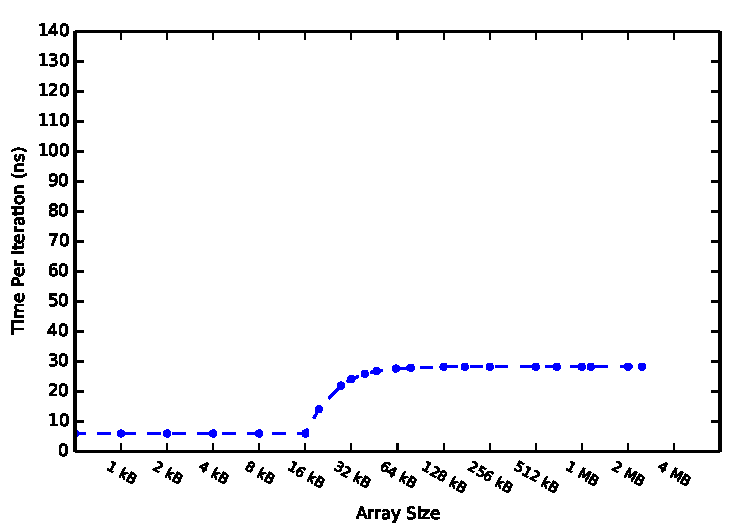
\includegraphics[width=\textwidth]{figures/ccbench_lat1.pdf}
% 	\caption{DRAM Latency = 1}
% \end{subfigure}
% \begin{subfigure}[t]{0.33\textwidth}
% 	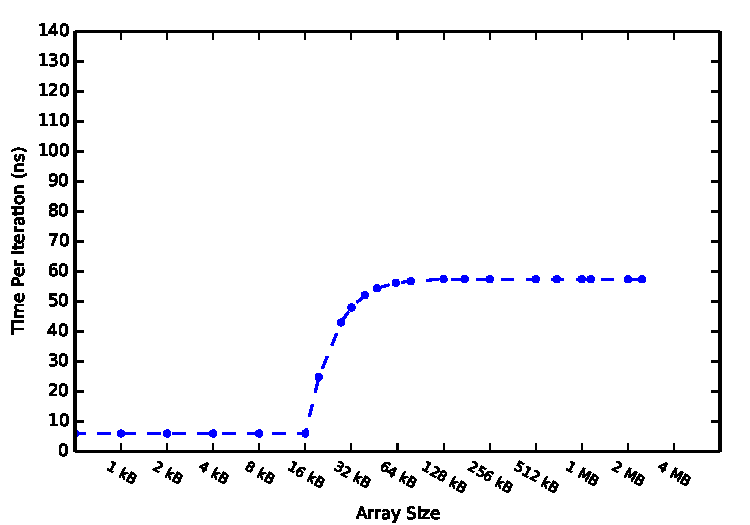
\includegraphics[width=\textwidth]{figures/ccbench_lat30.pdf}
% 	\caption{DRAM Latency = 30}
% \end{subfigure}
% \begin{subfigure}[t]{0.33\textwidth}
% 	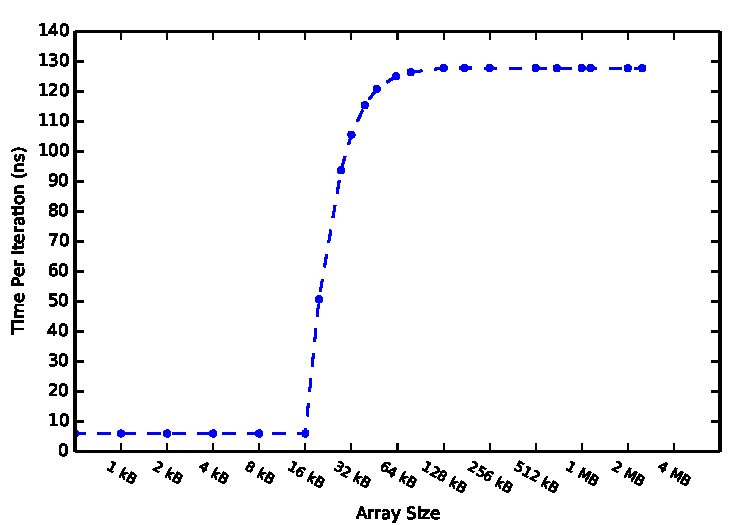
\includegraphics[width=\textwidth]{figures/ccbench_lat100.pdf}
% 	\caption{DRAM Latency = 100}
% \end{subfigure}
% \caption{Latency Validation}
% \label{fig:lat_val}
% \end{figure*}

% Figure~\ref{fig:lat_val} shows the results of cache hierarchy tests in \textit{ccbench}
% for BOOM-2w, assuming its frequency is 1GHz. We can see that the amount of
% the time per iteration with arrays bigger than the cache size observed by the target system
% increases by the delay of the off-chip memory as the DRAM latency increases.
% In this case, 1 cycle is 1ns, and thus, the time per iteration with large arrays
% increases by 30ns and 100ns as the DRAM latency increases by 30 cycles and 100 cycles,
% respectively.

Figure~\ref{fig:gcc_ref} shows how CPI varies over time for \textit{403.gcc} with the reference
input set running on the Rocket processor. We first measure the performance with a
magic memory with a one-cycle latency to determine the maximum performance the Rocket processor can
achieve. Next, we increase the memory latency to 30 cycles and see how much the Rocket processor
slows down.

This experiment demonstrates that our simulation methodology enables ``what-if'' experiments
regarding memory parameter configurations for very long-running applications, which is
practically impossible with software simulators. Note that the dynamic instruction count for
\textit{403.gcc} with the reference input is 1.3 trillion (Table~\ref{tbl:spec_ref}). The
effective simulation rate is 29 MHz on the FPGA, whose operating frequency is 40 MHz. The
simulation slow-down is due to the communication overhead between the software components and the
FPGA-based simulator.

\begin{figure*}
	\centering
	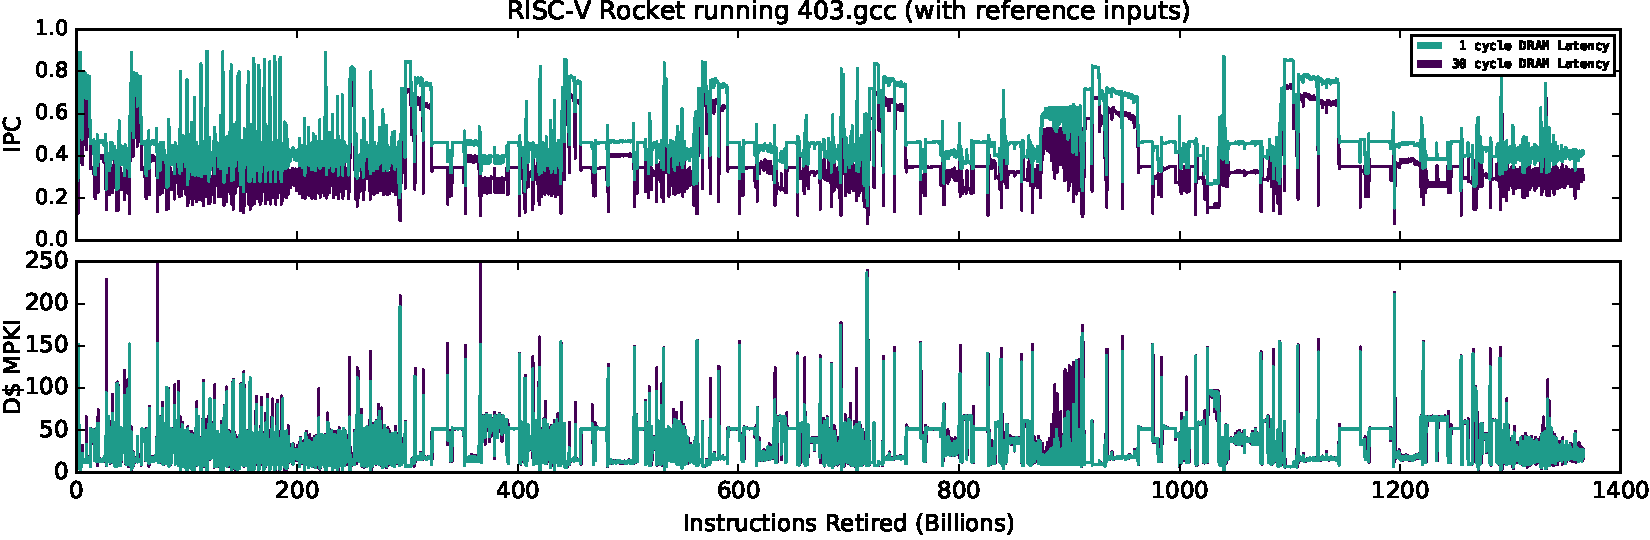
\includegraphics[width=0.95\textwidth]{figures/403-gcc-ref.pdf}
	\caption{CPI and D\$ MPKI for 403.gcc with the reference input running on the Rocket processor}
	\label{fig:gcc_ref}
\end{figure*}

\subsection{Bandwidth Configurations}

% \begin{figure*}
% \begin{subfigure}[t]{0.33\textwidth}
% 	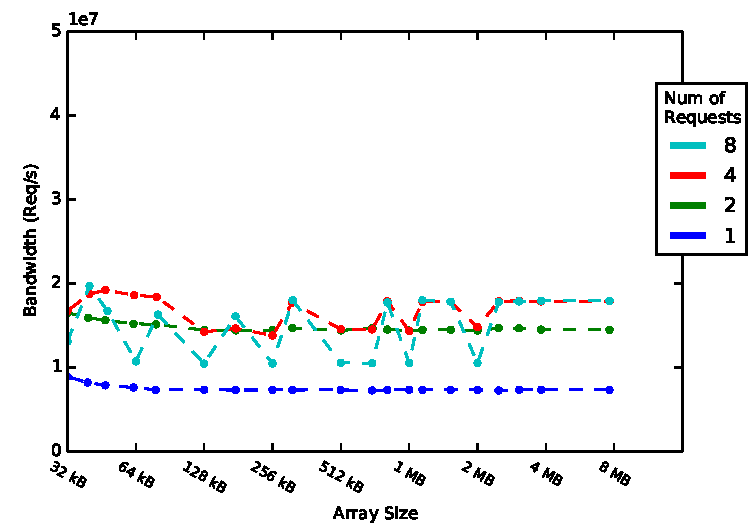
\includegraphics[width=\textwidth]{figures/ccbench_bw2.pdf}
% 	\caption{DRAM Bandwidth = 2}
% \end{subfigure}
% \begin{subfigure}[t]{0.33\textwidth}
% 	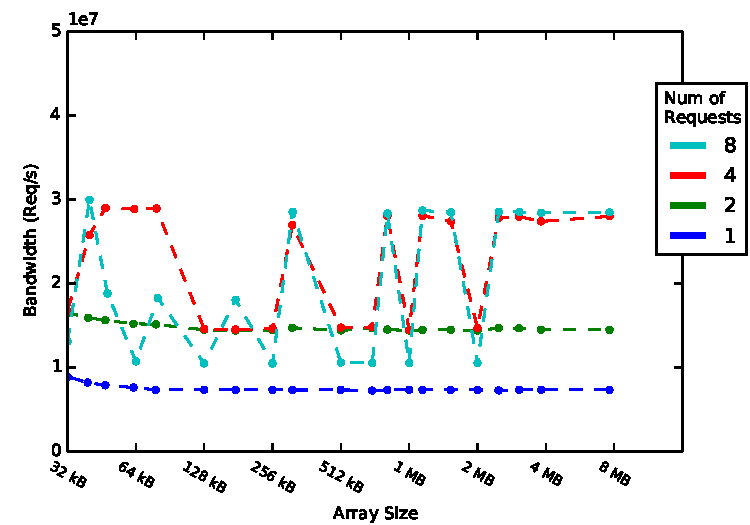
\includegraphics[width=\textwidth]{figures/ccbench_bw4.pdf}
% 	\caption{DRAM Bandwidth = 4}
% \end{subfigure}
% \begin{subfigure}[t]{0.33\textwidth}
% 	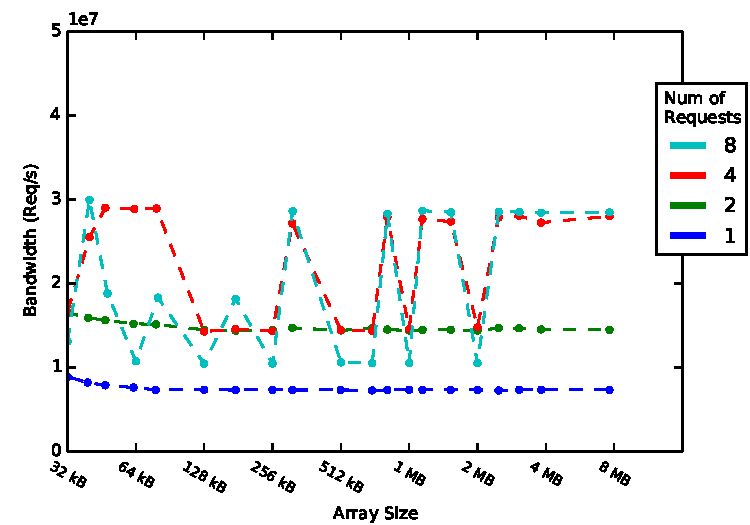
\includegraphics[width=\textwidth]{figures/ccbench_bw8.pdf}
% 	\caption{DRAM Bandwidth = 8}
% \end{subfigure}
% \caption{Bandwidth Validation}
% \label{fig:lat_val}
% \end{figure*}

\begin{figure}[t]
	\centering
	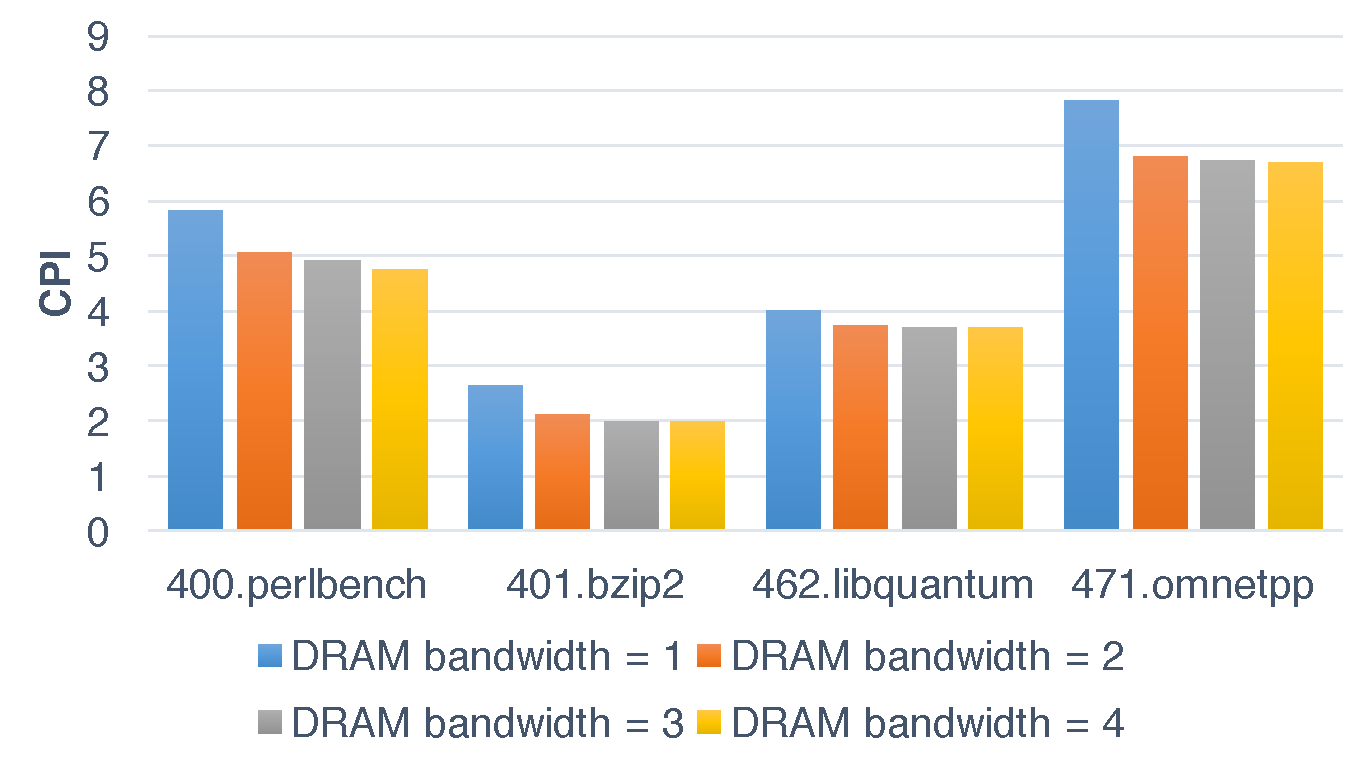
\includegraphics[width=0.8\columnwidth]{figures/boom-bw.pdf}
	\caption{CPIs for BOOM-2w with various bandwidths}
	\label{fig:bandwidths}
\end{figure}

Our next experiment highlights how various memory bandwidths affect the performance of
a superscalar out-of-order processor, assuming the DRAM latency is 100 cycles.
Figure~\ref{fig:bandwidths} shows CPIs for BOOM-2w with various bandwidth 
running \textit{401.bzip2}, \textit{462.libquantum}, and \textit{471.omnetpp}
with the test inputs.
We expect BOOM-2w to be able to issue more memory requests in flight than Rocket,
and thus, we believe memory bandwidth is an important parameter for this case study.
As seen in Figure~\ref{fig:bandwidths}, there is a significant performance
advantage when we increase the memory bandwidth from 1 to 2. However,
the performance benefits diminish as we increase the bandwidth further,
due to lack of memory-level parallelism in the benchmarks.

\subsection{Bank Conflict Model}

\begin{figure}[t]
	\centering
	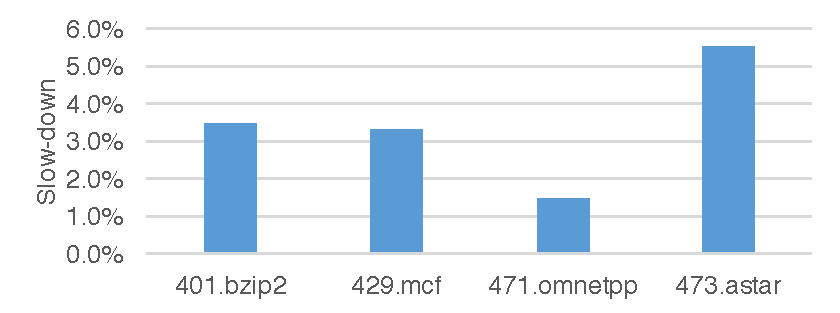
\includegraphics[width=0.8\columnwidth]{figures/boom-bc.pdf}
	\caption{Performance degradation from bank conflicts with 8 banks and a 20-cycle penalty}
	\label{fig:bank_conflict}
\end{figure}

Figure~\ref{fig:bank_conflict} shows how bank conflicts degrade the processor performance.
We run the benchmarks on BOOM-2w with a 8-bank DRAM by varying the bank conflict penalty 
from 1 cycle to 20 cycles. We can see the benchmarks suffer from performance degradation
due to bank conflicts as expected.

\subsection{FCFS MAS Model}

\begin{figure}[t]
		\centering
		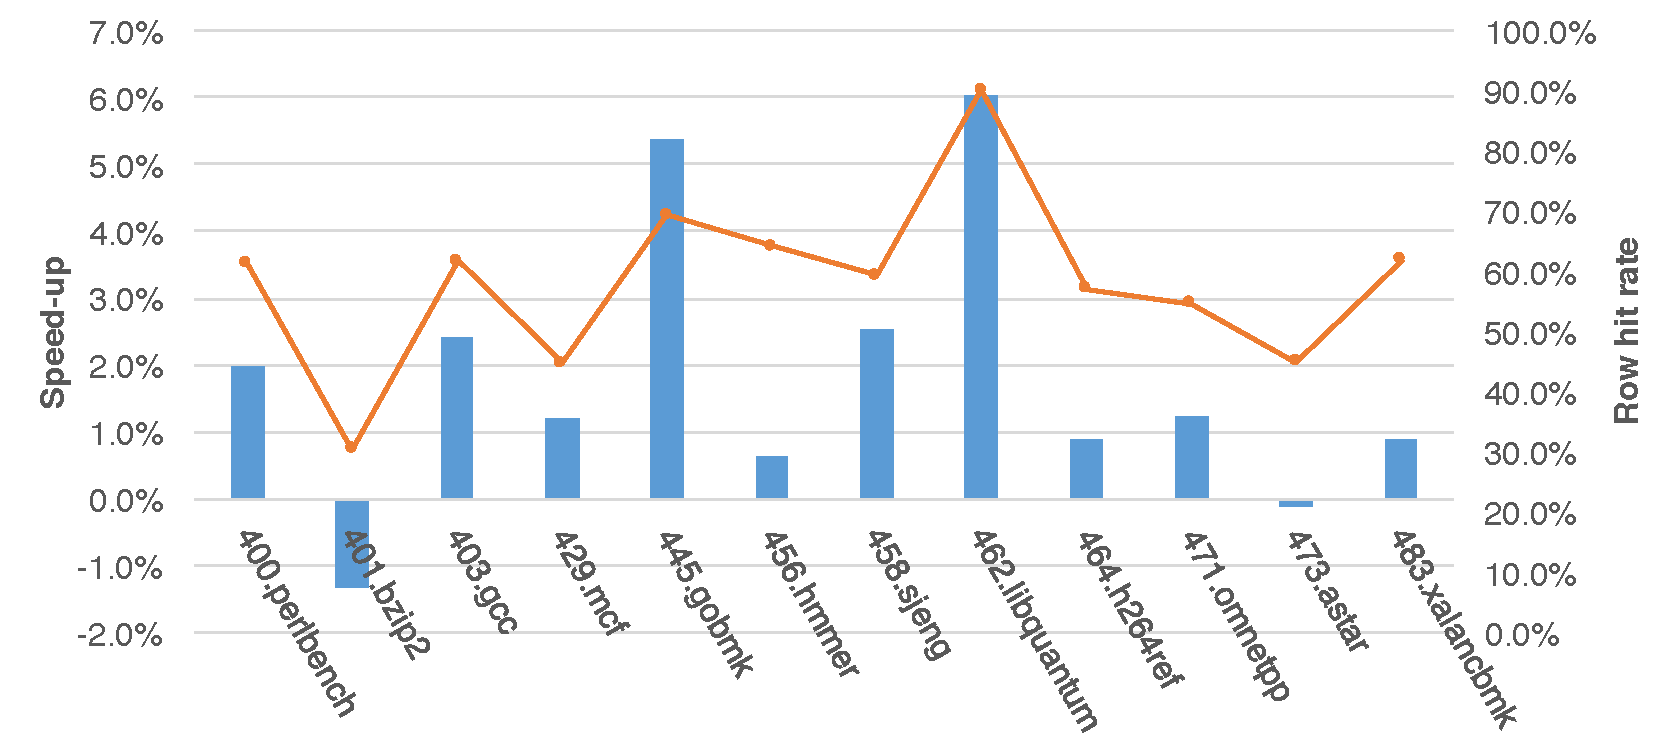
\includegraphics[width=\columnwidth]{figures/rocket-fifomas.pdf}
		\caption{Speedup of the open-page FCFS MAS policy over the close-page policy for Rocket}
		\label{fig:rocket_fifo_mas}
\end{figure}

This section shows the performance impacts of the page policies with the FCFS MAS model
(Section~\ref{sec:timing_model}). This represents a more complex policy, and we contrast variants with open and close row policies.

\begin{table}[t]
\centering
\resizebox{0.7\columnwidth}{!}{%
\begin{tabular}{|c|c c|}
\hline
\textbf{Parameter} & \textbf{Open Policy} & \textbf{Close Policy} \\
\hline
\textit{number of banks} & 8 & 8 \\
\textit{bank address offset} & \textbf{13} & \textbf{6} \\
\textit{row address offsets} & 16 & 16 \\
\textit{bandwidth} & 8 & 8 \\
\textit{tRC} & 7 cycles & 7 cycles \\
\textit{tRCD} & 7 cycles & 7 cycles\\
\textit{tCAS} & 7 cycles & 7 cycles \\
\hline
\end{tabular}}
\caption{FIFO MAS Parameters}
\label{tbl:fifo_mas}
\end{table}

Table~\ref{tbl:fifo_mas} lists the parameter values used in this experiment.
Figure~\ref{fig:rocket_fifo_mas} shows the speedup of the open page policy over the close page
policy for the SPEC benchmarks and the DaCapo benchmarks running on Rocket, along with the row
hit rate for each benchmark. Overall, the open page policy has perfomance benefits for the SPEC
CPU integer benchmarks except for \textit{402.bzip2} and \textit{473.astar}. As indicated in
Figure~\ref{fig:rocket_fifo_mas}, the memory requests of \textit{402.bzip2} and
\textit{473.astar} lack locality (resulting in low row hit rates), which explains these results.


\chapter{Conclusion}

FPGAs in the cloud provide a compelling platform to build fast, detailed
full-system simulators. However, if FPGA-accelerated simulation is to see wider
adoption, the usability limitations of prior work must be addressed.  One
promising avenue lies in automatically deriving cycle-exact, bit-exact FPGA
models from synthesizable target RTL modules. This reduces model-building and
validation effort while enabling researchers to also observe cycle-time, area,
and power impacts using commercial ECAD tools.

\PNAME addresses a longstanding hole in these RTL-transforming approaches by
providing models of outer cache hierarchies and DRAM memory systems---components
of the target design that cannot be naively transformed from ASIC
RTL.  However, by applying the same transformation on a target-time
timing-model, \PNAME obviates many of the pitfalls of handwriting FPGA-hosted
models, as it separates the concerns target-behavior modeling and
host-platform mapping. As a result, \PNAME instances are both fast---capable
of running at the host frequency---and detailed---comparable to
cycle-accurate software simulators of DRAM---while being far less onerous
to implement.


\printbibliography

\end{document}
